\section{ Overview}
For CKB platform we will use a three tier architecture. A three-tier architecture is a popular software application structure that divides applications into three distinct computing levels: the presentation layer, which is the user interface; the application layer, which is where data is processed; and the data layer, which is where the data related to the application is stored and managed. The main advantage of this architecture is that each tier can be developed and updated independently by a different development team, and can be scaled up or down without affecting the other tiers.\cite{threeTier}
\\
\\
\\
\begin{figure}[!h]
    \centering
    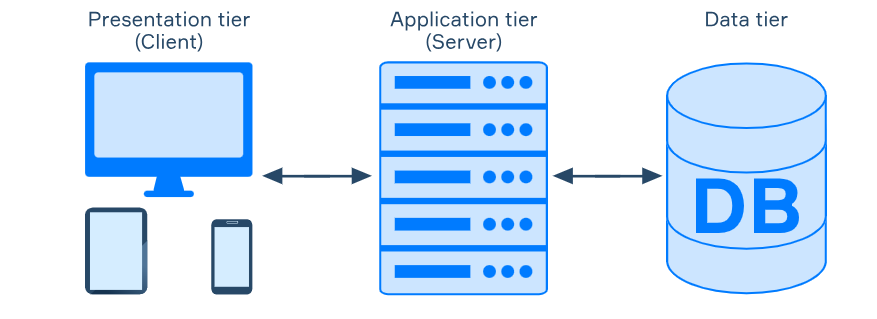
\includegraphics{Images/three tier architecture.png}
    \caption{Three tier architecture}\cite{three_Tier}
    \label{fig:three-tier}
\end{figure}

\subsection{Distributed view}
    \begin{figure}
        \centering
        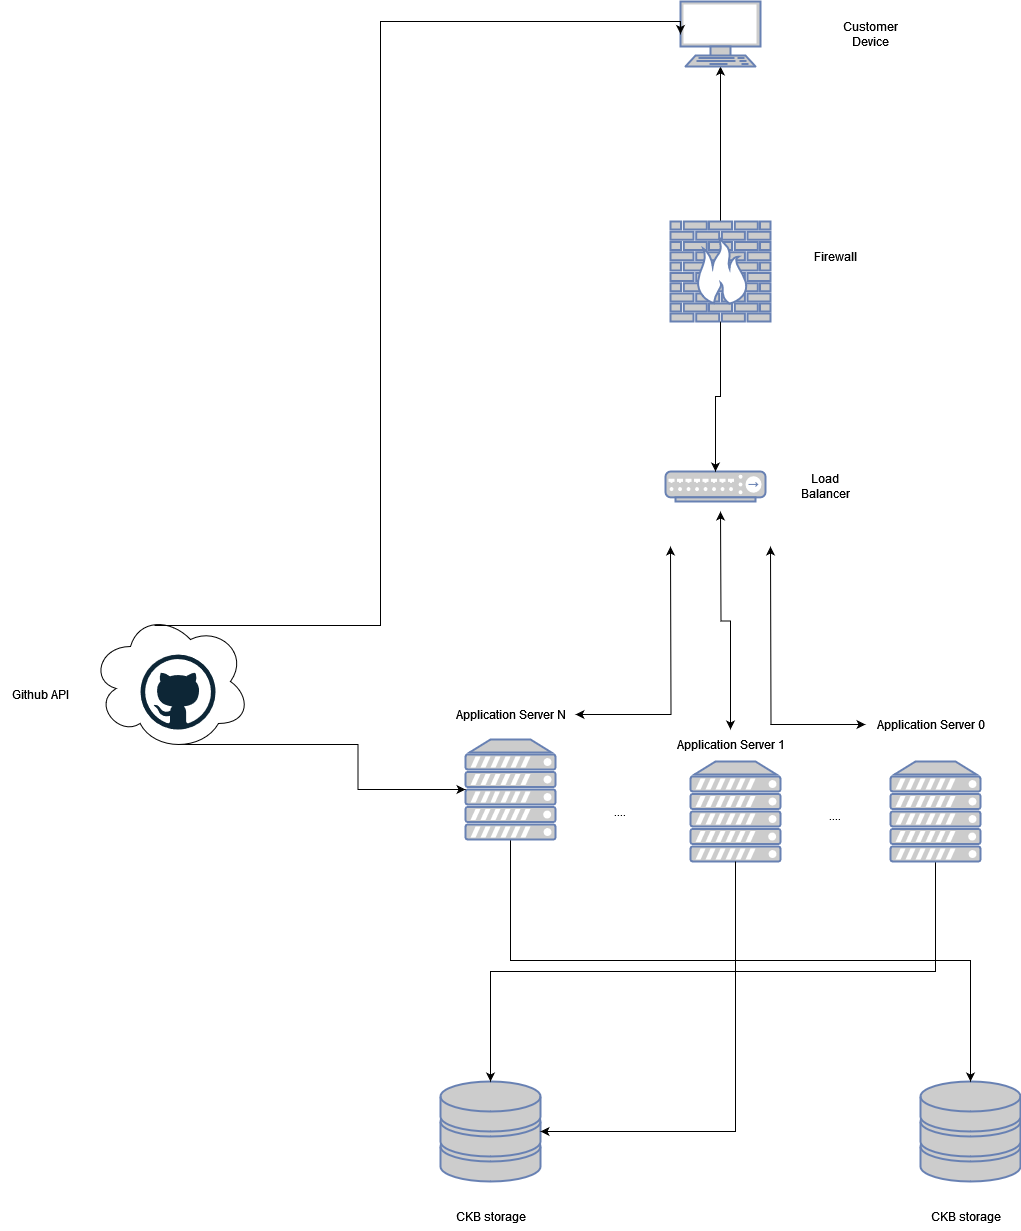
\includegraphics[width=\textwidth]{Images/DSV.drawio.png}
        \caption{Distributed view}
        \label{fig:enter-label}
    \end{figure}

\newpage
\section{Component view}
As mentioned for the platform we will use a three tier architecture. In figure \labelcref{fig:backend} it is possible to find the component view diagram of the platform. The back-end will implement an API which will be used by the web app (presentation layer). As you can see from the diagram, the data layer will also interact with the back-end, as will GitHub and the static analysis tool. The main components of the back-end are:
\begin{itemize}
    \item AuthenticationManager: provides the functionalities related to the authentication of the users to GitHub
    \item AccountManager: provides the functionalities related to the users general information and profile
    \item TeamManager: provides the functionalities related to the management of teams, necessary so students can participate in the battles.
    \item CompetitionStructureManager: This will implement the organizational part of the competition
    \item CompetitionEvaluationManager: Implements the evaluation of the competition. On contrast with the previous one, it is more dynamic because is triggered on every commit and it is also more computational intensive as it performs all the calculations needed for computing the score, the ranking and in order to assign the badges.
    \item DynamicAnalyser: implements the dynamic analysis tool that will run the test on the code submitted by the students. Because malicious users might try to exploit some vulnerability by providing malicious tests or code, we keep it separate from the previous.
    \item NotificationManager: Implements whats necessary so the platform can send notifications when needed
    \item Database: stores all the data of the app (Data Layer)
    \item API: The main purpose is to expose an API for the webApp, routing the incoming request to the appropriate internal component.

    For the front-end, the main component is:
        \begin{itemize}
            \item WebApp: The client app with which users will interact directly. Apart from the user interface it will contain some logic necessary to interact efficiently with the back-end REST API
        \end{itemize}
\end{itemize}

\newpage
\begin{figure}[!h]
    \centering
    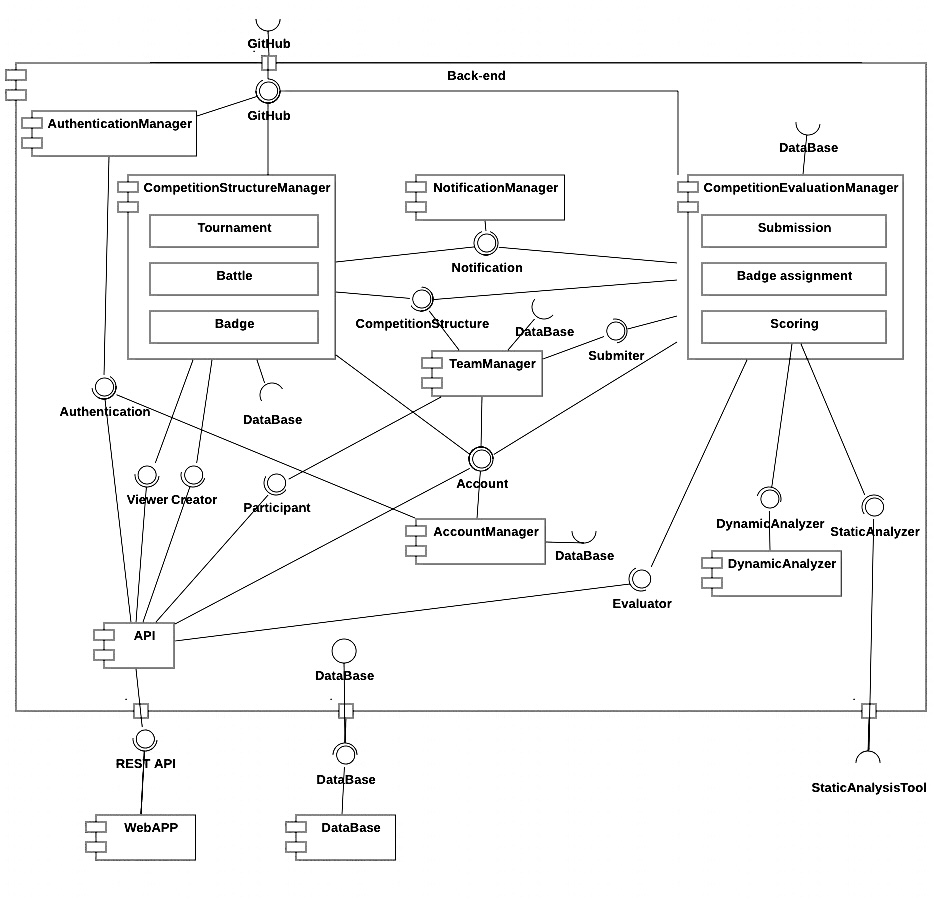
\includegraphics[width=\textwidth]{Images/Backend.jpeg}
    \caption{Component view}
    \label{fig:backend}
\end{figure}

\pagebreak
\section{Deployment view}
Here is showed the deployment view which is important because it describes the execution environment of the system but it also shows the topological distribution of the CKB application


\begin{figure}[!h]
    \centering
    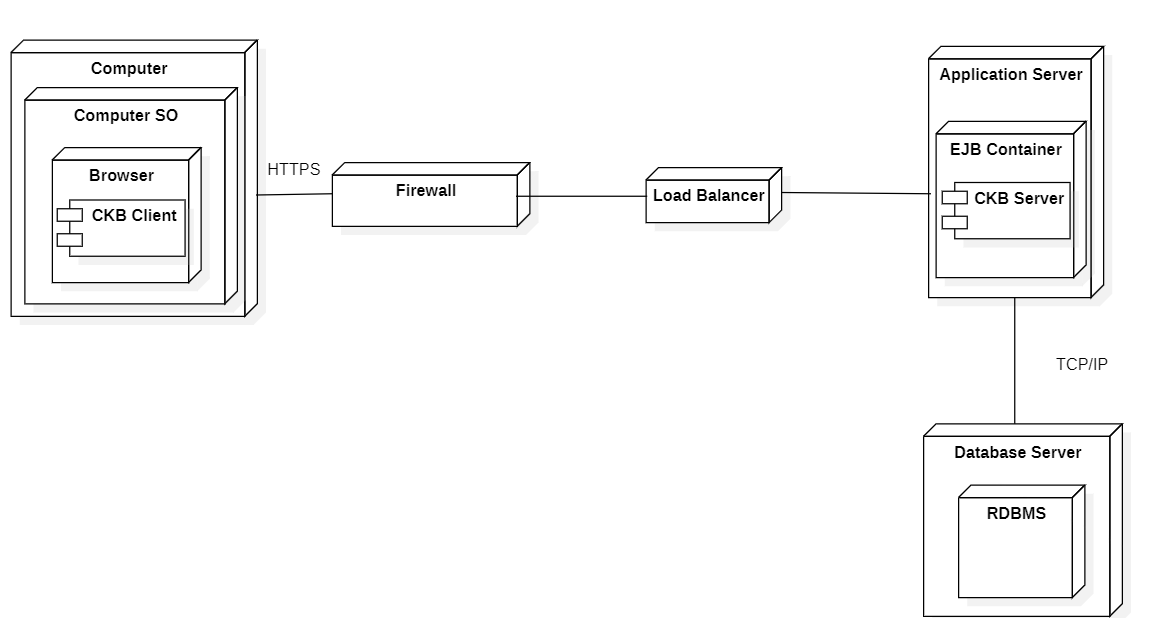
\includegraphics[width=\textwidth]{Images/Deployment_DIagram.png}
    \caption{Deployment view diagram}
    \label{fig:dep}
\end{figure}

The device SO is the one in which the browser is running from the browser it is possible to start the client-side app then every client request is processed by a firewall which is in charge of checking if some malicious request are sent to the server. A load balancer is a device useful for avoiding brute force attack to the server and, in general to not overload the server cpu capacities with a lot of request to process.The application server is able to manage the software architecture on the server-side then every change in the database is updated by the application server via TCP/IP.


\section{Runtime view}
\begin{enumerate}[label=\textbf{[UC\arabic*]}]
    \begin{figure}
    \item \textbf{User Registration}
        \centering 
        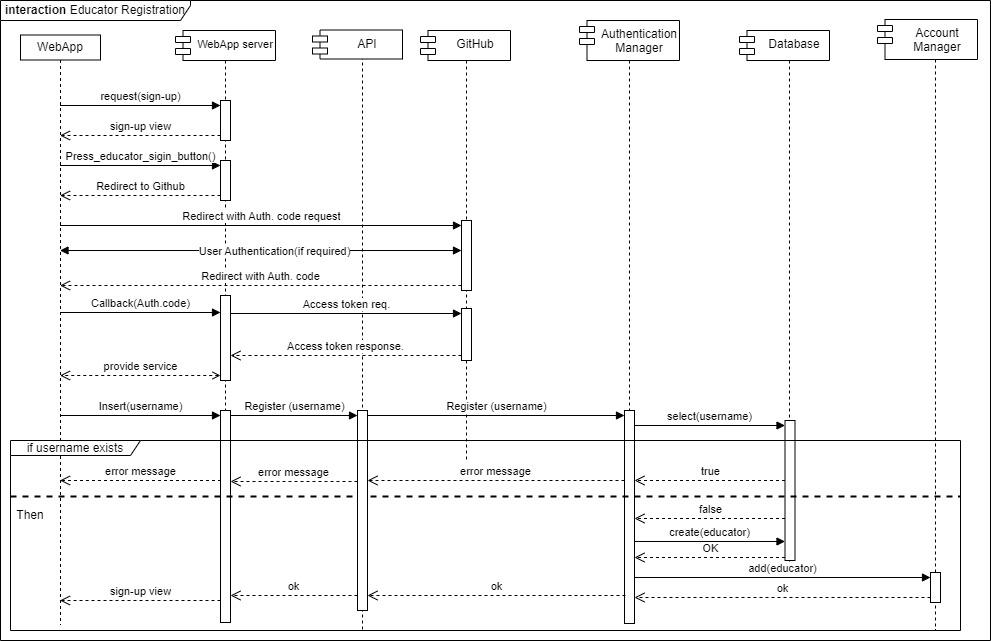
\includegraphics[width=\textwidth]{Images/User_registration.jpg}
        \caption{User Registration}
        \label{fig:enter-label}
        \raggedright The figure shows the process of the sign-in of the educator.
        Once it is sent the request to sign-up with GitHub, it will start the process of authentication, managed by the authentication manager. 
        GitHub handles authenticated requests after the application has obtained an access token.
        When the process of authentication is completed, the educator fills the educator profile form with the information needed to create the profile of the user who is signing up. 
        As soon as the form is submitted and sent to the authentication manager, it is asked to the database to check whether the username already exist in the platform. Then if the chosen username is new the database stores the information of the educator and the account manager adds the user to the table of educators.

        The process is the same for the student sign-up, however it is sent a different request from the browser to the webapp server. Another difference lies in storing student information that is separate from that of the educator. 
    \end{figure}

    \begin{figure}
    \item \textbf{User Login}
        \centering
        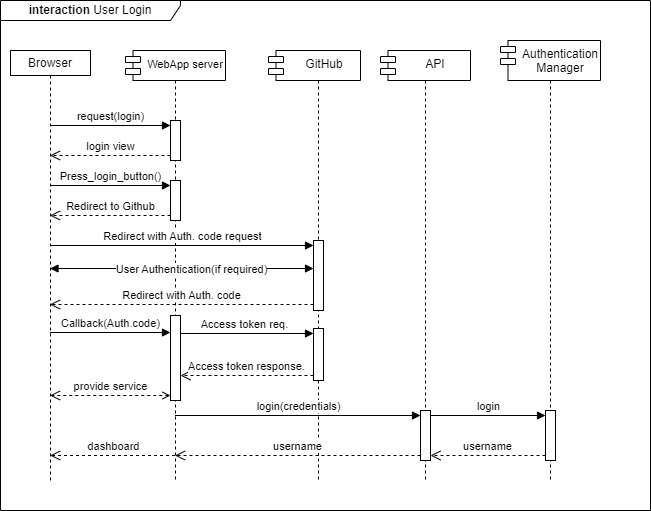
\includegraphics[width= \textwidth]{Images/User_login (1).jpg}
        \caption{User Login}
        \label{fig:enter-label}
        \raggedright The figure shows the process of login of a user. Since the information of both students and educators have been separately stored in the database, the process of login is the same for both of the two figures. 
        The login is managed by GitHub. Once the webapp has obtained the access token the webapp can check the credentials thanks to the authentication manager and let the user log to the platform.
    \end{figure}

    \begin{figure}
    \item \textbf{Tournament Creation}
        \centering
        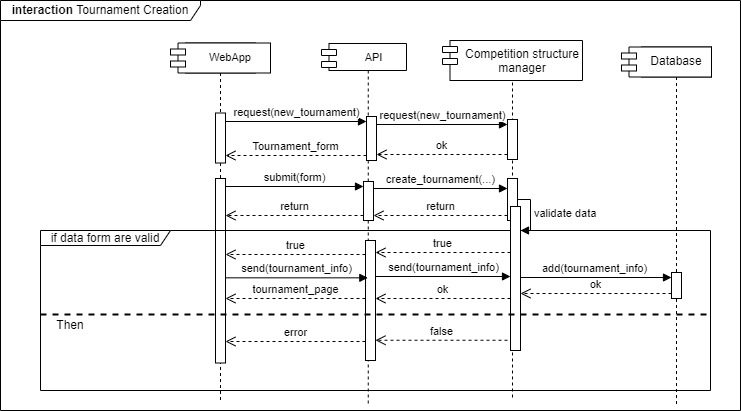
\includegraphics[width= \textwidth]{Images/Tournament_creation.jpg}
        \caption{Tournament Creation}
        \label{fig:enter-label}
        \raggedright This figure shows the process of the creation of the tournament. the user send to the WebApp  a request of creation of a new tournament. As a consequence the form is shown and it is filled with the tournament information. Then the competition structure manager is in charge of the validation of the information sent, if the information are valid they are inserted into the database.
    \end{figure}
    
    \begin{figure}
    \item \textbf{Battle Creation}
        \centering
        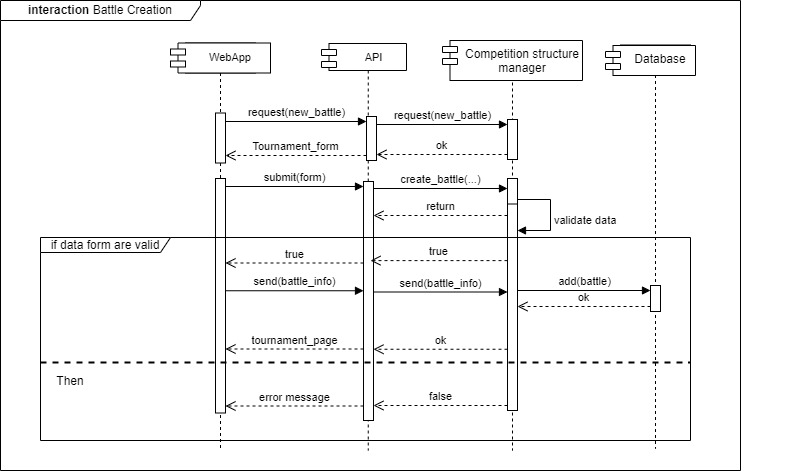
\includegraphics[width= \textwidth]{Images/Battle_creation.jpg}
        \caption{Battle Creation}
        \label{fig:enter-label}
        \raggedright The figure shows the process of the creation of a battle. As for the previous case, the user send to the WebApp  a request of creation of a new battle. So the form is shown and it is filled with the battle information. Then the competition structure manager is in charge of the validation of the information sent, if the information are valid they are insert into the database, in order to create the battle.
    \end{figure}
    
    \begin{figure}
    \item \textbf{Add collaborator}
        \centering
        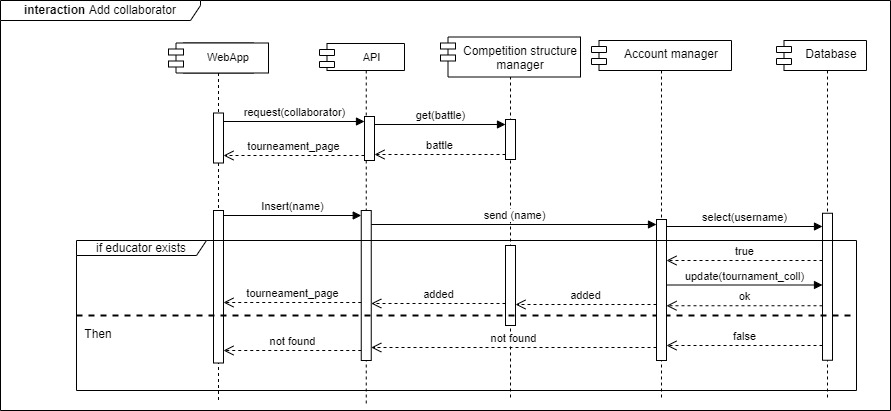
\includegraphics[width= \textwidth]{Images/Add_collaborator.jpg}
        \caption{Add collaborator}
        \label{fig:enter-label}
        \raggedright The figure shows the process of adding another educator to a tournament. The request is sent form the user to the competition structure manager which is in charge of return the tournament where the educator will be added.
        Then the user types the name of the user to add, then the account manager will request to the database to check whether the name inserted by the user is an educator. If yes the collaborator is added to the tournament collaborators.
    \end{figure}
    
    \begin{figure}
    \item \textbf{Team Creation}
        \centering
        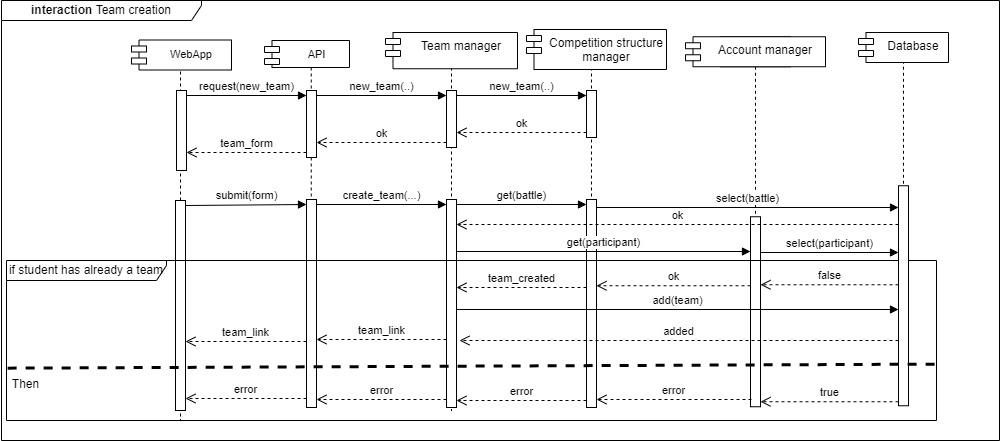
\includegraphics[width= \textwidth]{Images/Team_creation.jpg}
        \caption{Team Creation}
        \label{fig:enter-label}
        \raggedright The figure shows how a team is created. The student request the creation of a new team managed by the team manager. When the form is submitted, the team manager request to the competition structure manager the battle in order to associate the battle with it. In the end the competition structure manager has to check whether the user who request a team is a student already enrolled in a team. Once when it has been verified then it inserts the team into the database.
    \end{figure}
    
    \begin{figure}
    \item \textbf{Join Team}
        \centering
        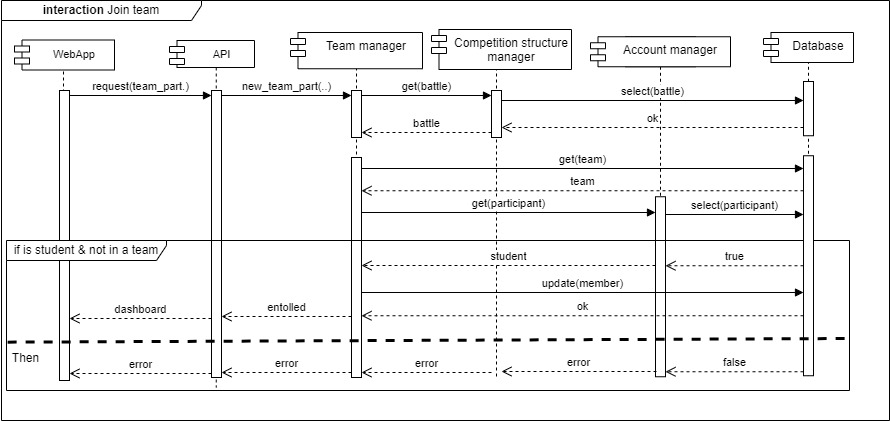
\includegraphics[width= \textwidth]{Images/Join_team.jpg}
        \caption{Join Team}
        \label{fig:enter-label}
        \raggedright The figure shows how a student that has already received a link can join a team. Once the link has been opened, the webapp send a request to the team manager to join the team. The manager asks the competition structure manager to get the battle information, then recover the information of the team associated to such battle. Then the manager check if the user is registered to the platform and and is not enrolled in other teams.
    \end{figure}
    
    \begin{figure}
    \item \textbf{Battle Begins}
        \centering
        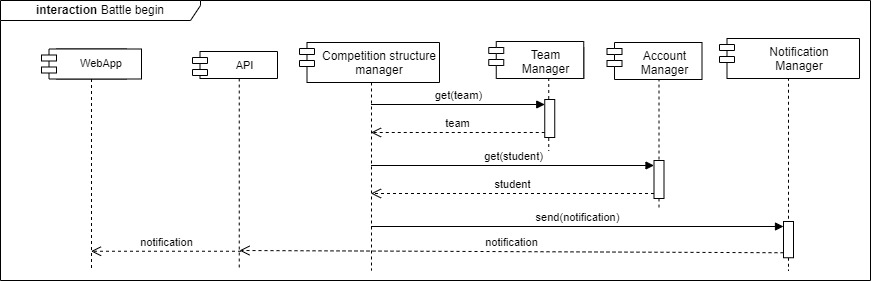
\includegraphics[width= \textwidth]{Images/Battle_begin.jpg}
        \caption{Battle Begins}
        \label{fig:enter-label}
        \raggedright The figure shows of the battle starts. As said in the RASD the battle starts as soon as the the enrollment deadline of the battle ended. Then the competition structure manager selects the students or the teams enrolled in such battle so that it can request to the notification manager to notify them.
    \end{figure}
    
    \begin{figure}
    \item \textbf{Code submission}
        \centering
        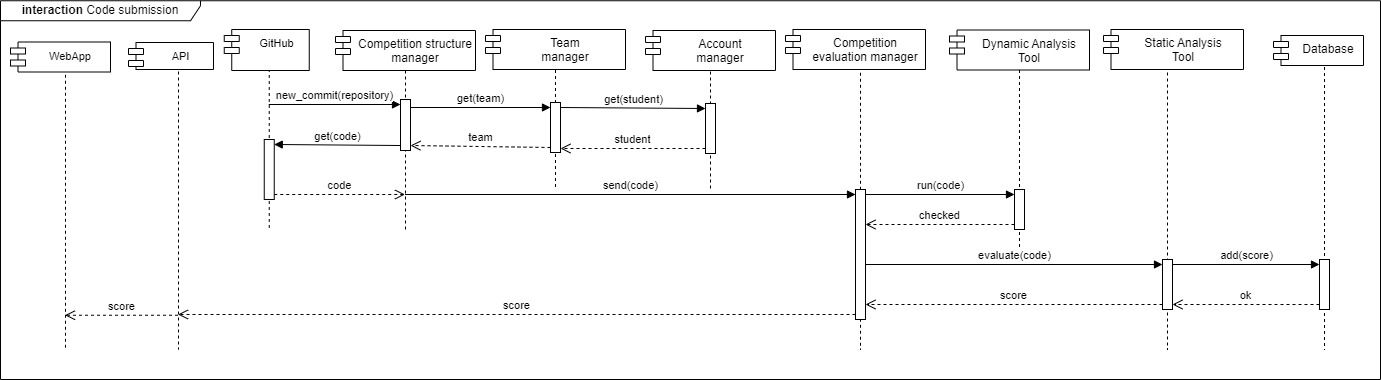
\includegraphics[width= \textwidth]{Images/Submits_code.jpg}
        \caption{Code submission}
        \label{fig:enter-label}
        \raggedright The figure shows the process of submission of a code from a certain team. The competition structure manager is triggered by GitHub as soon as a new commit has been done, as a consequence it looks for the team and its participants, in order to associate the code to the team. Then through a callback the manager gets the code so that it can be sent to the competition evaluation manager which is in charge of request to the dynamic analysis tool to check the code. Once the code has been checked the manager request the evaluation to the static analysis tool. The resulting score will be added to the database and sent to the webapp.
    \end{figure}

    \begin{figure}
    \item \textbf{The battle ends}
        \centering
        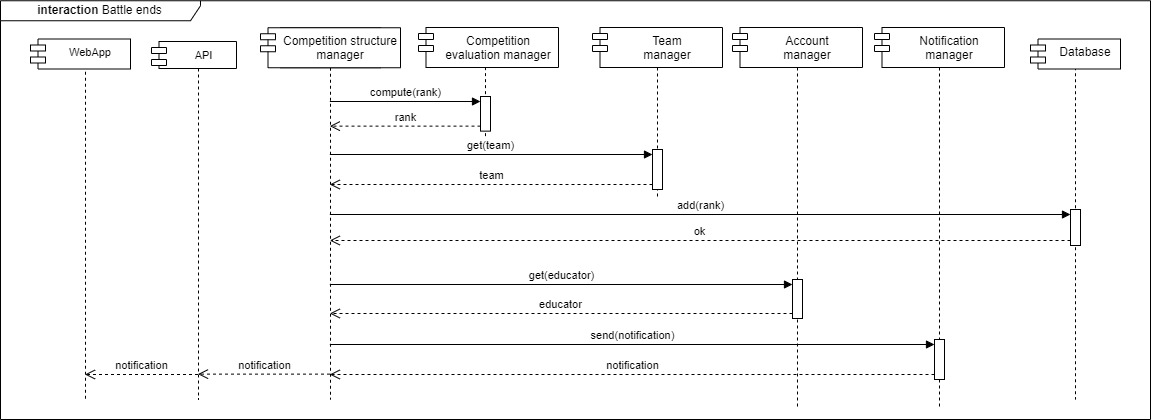
\includegraphics[width= \textwidth]{Images/Battle_ends.jpg}
        \caption{The battle ends}
        \label{fig:enter-label}
        \raggedright The figure shows how is it managed the end of a battle. The competition structure manager ask the competition evaluation manager to compute the rank of the battle, than request the team manager to get the team in order to associate the ranks to the teams and store it in the database. In the end it ask the notification manager to notifies students about the new rank.
    \end{figure}
    
    \begin{figure}
    \item \textbf{Code Evaluation}
        \centering
        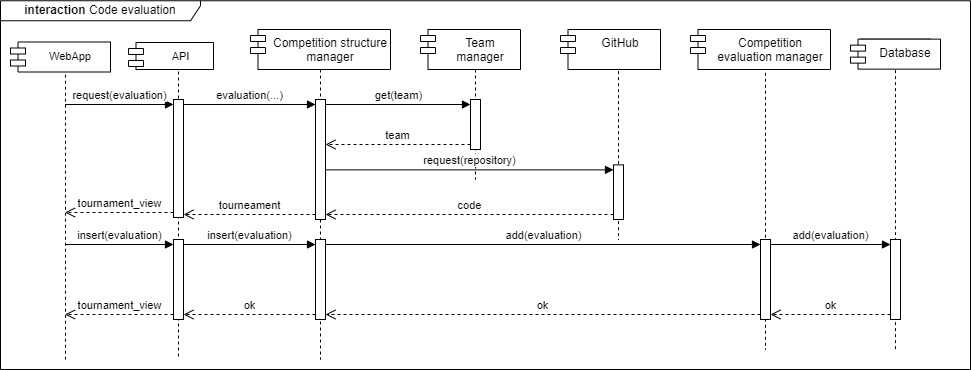
\includegraphics[width= \textwidth]{Images/Code_Evaluation.jpg}
        \caption{Code Evaluation}
        \label{fig:enter-label}
        \raggedright The figure shows the process of manual evaluation done by the educators at the end of the tournament,if necessary. The consolidation phase started. The webapp request the competition structure manager for a manual evaluation, as a consequence the manager request the team to the team manager and the code from GitHub which retrieves it through the repository. Then the user can inset his evaluation in the platform which will be sent to the competition structure manager and the competition evaluation manager and finally stored in the database.
    \end{figure}

    \begin{figure}
    \item \textbf{Publish Final Rank}
        \centering
        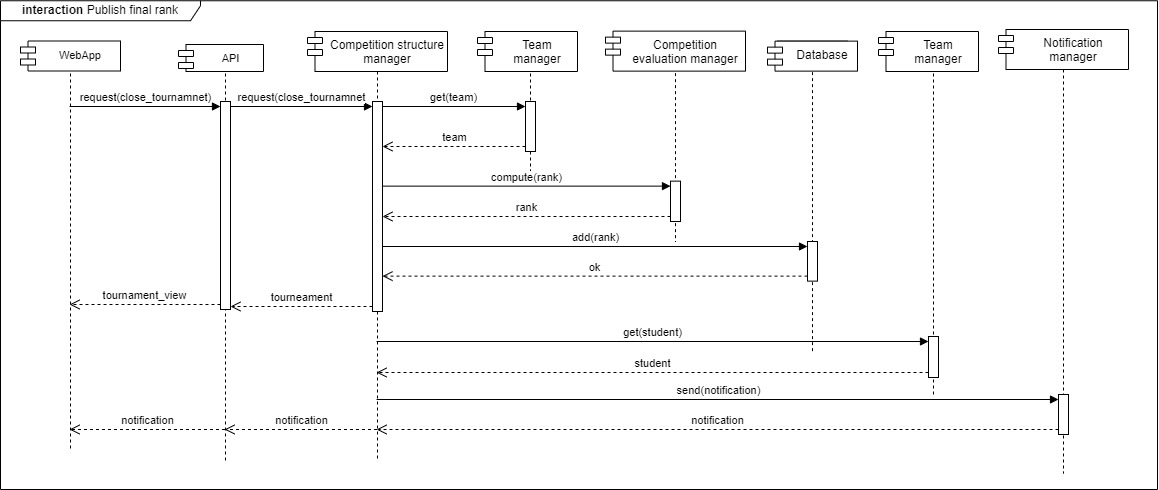
\includegraphics[width= \textwidth]{Images/Publish_Final_Rank.jpg}
        \caption{Publish Final Rank}
        \label{fig:enter-label}
        \raggedright The figure shows the process of closure of the tournament. When the educator closes the tournament, the competition structure manager takes care of recovering the name of the team and asks the competition evaluation manager to calculate the final rank and so updates the rank in the database.
        After that the competition structure manager is in charge of notify the student about the final rank update. Asks the account manager the name of the student who will receive the notification from the notification manager.
    \end{figure}

    \begin{figure}
    \item \textbf{See Profile}
        \centering
        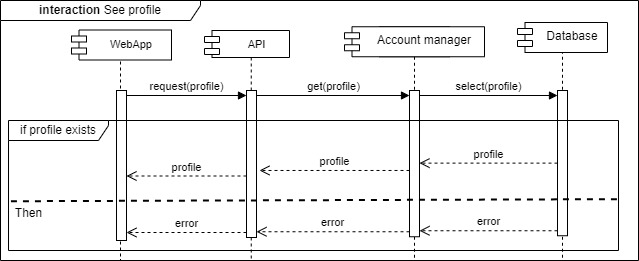
\includegraphics[width= \textwidth]{Images/See_Profile.jpg}
        \caption{See Profile}
        \label{fig:enter-label}
        \raggedright The figure shows how the user can look for a profile of a user in the platform. As soon as the name is searched, is sent a request of getting a profile to the account manager, which ask the database to check whether the name is a user of the platform.
    \end{figure}
    \begin{figure}
    \item \textbf{Badge Creation}
        \centering 
        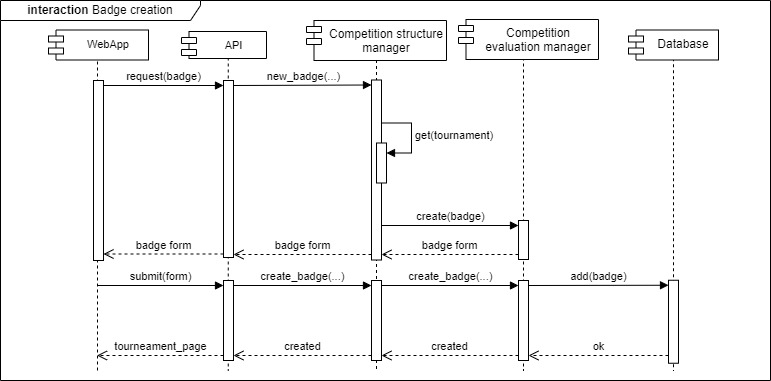
\includegraphics[width= \textwidth]{Images/Badge_Creation.jpg}
        \caption{Badge Creation}
        \label{fig:enter-label}
        \raggedright The figure shows the creation of a badge. The request is sent to the competition structure manager which gets the tournament associated to the badge. When the form of the badge has been submitted, the competition structure manager forward the request of creation of the badge to the competition evaluation manager and then the badge is added to the database.
    \end{figure}
\end{enumerate}
\pagebreak

\section{ Component interfaces}

    \subsubsection{WebApp server}
    \begin{itemize}
        \item request(sign-up)
        \item press educator sigin button()
        \item callback(Auth.code)
        \item request(login)
        \item Press login button()
    \end{itemize}
    
    \subsubsection{GitHub}
    \begin{itemize}
        \item redirect with Auth. code request
        \item access token req.
        \item request(repository)
    \end{itemize}
    
    \subsubsection{API}
    \begin{itemize}
        \item register (username)
        \item login(credentials)
        \item login
        \item request(new tournament)
        \item submit(form)
        \item send(tournament info)
        \item request(new battle)
        \item send(battle info)
        \item request(collaborator)
        \item insert(name)
        \item request(new team)
        \item request(evaluation)
        \item insert(evaluation)
        \item request(close tournament)
        \item request(profile)
        \item request(badge)
    \end{itemize}
    
    \subsubsection{AuthenticationManager}
    \begin{itemize}
        \item register (username)
    \end{itemize}
    
    \subsubsection{CompetitionStructureManager}
    \begin{itemize}
        \item request(new tournament)
        \item send(tournament info)
        \item validate data
        \item request(new battle)
        \item get(battle)
        \item new team(...)
        \item request(team part.)
        \item new get(student)commit(repository)
        \item evaluation(...)
        \item insert(evaluation)
        \item request(close tournament)
        \item new badge(...)
        \item get(tournament)
        \item create badge(...)
    \end{itemize}
    
    \subsubsection{CompetitionEvaluationManager}
    \begin{itemize}
        \item send(code)
        \item compute(rank)
        \item add(evaluation)
        \item create(badge)
        \item create badge(...)
    \end{itemize}
    
    \subsubsection{NotificationManager}
    \begin{itemize}
        \item send(notification)
    \end{itemize}
    
    \subsubsection{TeamManager}
    \begin{itemize}
        \item new team(...)
        \item create team(...)
        \item new team part(...)
        \item get(team)
    \end{itemize}
    
    \subsubsection{AccountManager}
    \begin{itemize}
        \item select(username)
        \item add(educator)
        \item add(student)
        \item send (name)
        \item get(participant)
        \item get(student)
        \item get(educator)
        \item get(profile)
    \end{itemize}
    
    \subsubsection{DynamicAnalyzer}
    \begin{itemize}
        \item run(code)
    \end{itemize}
    
    \subsubsection{StaticAnalysisTool}
    \begin{itemize}
        \item evaluate(code)
    \end{itemize}
    
    \subsubsection{Database}
    \begin{itemize}
        \item create(educator)
        \item create(student)
        \item add(tournament info)
        \item add(battle)
        \item select(username)
        \item update(tournament coll)
        \item select(battle)
        \item select(participant)
        \item add(team)
        \item get(team)
        \item update(member)
        \item add(score)
        \item add(rank)
        \item add(evaluation)
        \item select(profile)
        \item add(badge)
    \end{itemize}

\pagebreak
\section{Selected architectural styles and patterns}
\subsection{3-tier Architecture}
The architectural style that is used is the 3-tier architecture style because it provides many benefits the main one is the modularization in three independent layers:

            \begin{itemize}
                \item  The \textbf{ web server}:is the presentation tier and provides the user interface.This is usually a web page or a web site.The content can be static or dynamic, and is usually developed using HTML, CSS and Javascript.
                \item The \textbf{application server}:it is the middle tier, implementing the business logic.
                \item The \textbf{database server}:it is the backend tier of a web application. It runs on DBMS, such as MySQL.
            \end{itemize}

\subsection{Model View Controller Pattern }
The CKB is basically a web application that allows users to have access to the CKB features.So The MVC pattern is the the best choice to implement the application:

    \begin{itemize}
        \item  \textbf{Model}:it manages the data, logic and rules of the application.
        \item  \textbf{View}:representation of information such as a chart. Multiple views of the same information are possible, such as a bar chart for management and a tabular view for accountants. 
        \item   \textbf{Controller}:it accepts input and converts it into commands for Model and view.
    \end{itemize}
    
The tasks division between these three elements provide a  strong decoupling which gives some benefits such as reliability, re usability .      

\subsection{Facade Pattern}
The facade pattern is a software design pattern that is useful for implementing the requests dispatching.In fact, the facade is an object that hides the more complex underlying. it improves the readability and usability of a software library by masking interaction with more complex components behind a single  API. it provides a context-specific interface to more generic functionality and it serves as a launching point for a broader refactor of monolithic or tightly-coupled systems in favor of more loosely-coupled code.
 
\section{Other design decisions}
In this section are explained some design decisions that have been taken in order to make the system work

\subsection{Availability}
The concept of Load Balancing has been introduced to design a system which is highly available and to be able to manage an high amount of request at the same time.it's also important to have some sort of replication to avoid a single point of failure.

\subsection{Data Storage}
The data storage is managed by using a database to store  the personal data of educator and students. Moreover, are used some additional data structure to have better query performances 

\subsection{Security}
The security is managed by means of a firewall that is necessary to filter some cyber attacks.


